\documentclass[tikz,border=2pt]{standalone}
\usepackage{amsmath,amssymb}
\usepackage{tikz}

\begin{document}
% Shortest path from A to F: among all A-F paths the one of least total length,
% A-C-B-D-E-F with length 13 (compare A-B-D-F: 15, A-C-E-F: 15).
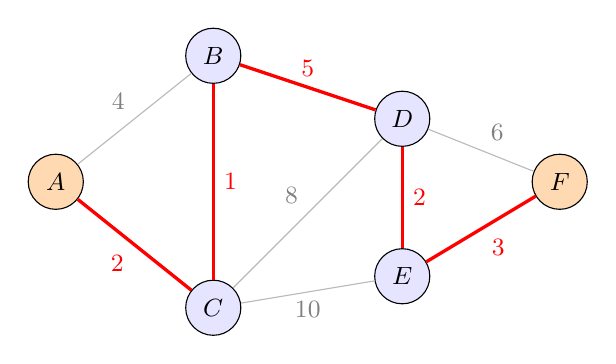
\begin{tikzpicture}[every node/.style={font=\small}, v/.style={draw, circle, fill=blue!10, minimum size=7mm, inner sep=0pt}]
	\node[v, fill=orange!30] (A) at (0,0) {$A$};
	\node[v] (B) at (2,1.6) {$B$};
	\node[v] (C) at (2,-1.6) {$C$};
	\node[v] (D) at (4.4,0.8) {$D$};
	\node[v] (E) at (4.4,-1.2) {$E$};
	\node[v, fill=orange!30] (F) at (6.4,0) {$F$};
	\draw[gray!55] (A) -- (B) node[midway, above left, font=\small, gray] {$4$};
	\draw[gray!55] (C) -- (D) node[midway, above left, font=\small, gray] {$8$};
	\draw[gray!55] (C) -- (E) node[midway, below, font=\small, gray] {$10$};
	\draw[gray!55] (D) -- (F) node[midway, above right, font=\small, gray] {$6$};
	\draw[red, very thick] (A) -- (C) node[midway, below left, font=\small] {$2$};
	\draw[red, very thick] (C) -- (B) node[midway, right, font=\small] {$1$};
	\draw[red, very thick] (B) -- (D) node[midway, above, font=\small] {$5$};
	\draw[red, very thick] (D) -- (E) node[midway, right, font=\small] {$2$};
	\draw[red, very thick] (E) -- (F) node[midway, below right, font=\small] {$3$};
	\end{tikzpicture}
\end{document}
